\chapter{Event Simulation and Reconstruction}

\section{Simulation} \label{sec:simulation}

To properly understand and interpret results, comparisons to theoretical prediction must be made. In the context of particle colliders, this means an understanding of both the underlying process as well as predictions of detector effects. To do this, a simulation framework has been developed. The framework is a serial process starting with event generation, those events then undergo parton showering, hadronization, detector simulation, and reconstruction.

At each step, a \gls{MC} integration is performed. A \gls{MC} simulation attempts to model a complex process by taking a function's underlying probability distribution and sampling it randomly {\color{red}}. Furthermore, when a process can be factorized, meaning it evolves serially, with each step dependent on only the prior, a method called \gls{MCMC}.

The evolution is described in the following sections, proceeding in steps of event generation, parton showering, hadronization, and finally detector simulation.

\noindent\textbf{Event Generation}\\
\indent The first step of the ATLAS simulation is generating the hard-scatter process. At the \gls{LHC}, in $pp$ collisions, the object ultimately collided are partons, the constituent strongly interacting particles (quarks and gluons) that comprise the protons. When simulating collisions, parton distribution functions are used, which describe the probability of finding a parton carrying a given fraction of the proton momentum.


Event generators produce \textit{matrix elements}, which take into account the partonic cross-section to a specified order approximation. The matrix element is returned in the \textit{Les Houches Accord} format \cite{les-houches}, which was designed to create a uniform event generator output. This format can then be interfaced to tools for parton shower and hadronization.

The ATLAS software contains many event generators. For the samples used in the presented analysis, the following generators are used:

\begin{description}
    \item \HERWIGpp: A general-purpose event generator \cite{herwigpp}
    \item \MADGRAPH: A matrix element generator, generating tree-level matrix elements for Lagrangian-based models \cite{mg5}
    \item \PYTHIA: A standard event generator \cite{pythia8.2}
    \item \POWHEG: A \gls{NLO} event generator that is built to overcome the problem of negatively weighted events \cite{powheg} % Used for vbf resonant samples, check if used otherwise
    \item \SHERPA: A general-purpose simulation tool, containing all necessary components for a factorized description of scattering events \cite{sherpa2.2}
\end{description}

\noindent\textbf{Parton Showering}\\
\indent Parton showering 

After interacting, the parton showering must then be simulated. Parton showering matches \gls{QCD} radiation to the matrix element 

% pick one of these
Several of the event generators in the ATLAS software have parton shower built in, notably among these \PYTHIA, \HERWIG, and \SHERPA.

There are two parton shower generators generally used in the ATLAS simulation software, \PYTHIA and \HERWIG. \PYTHIA orders its showers by $p_{T}$. \HERWIG utilizes angular ordering, to account for coherence effects. 

\noindent\textbf{Hadronization}\\
\indent Once partons have reached sufficiently low energies, they form hadrons. This is known as hadronization. Event generators implement models that are tuned on data. Commonly used are the Lund string model \cite{lund-string} (\PYTHIA) or clustering models \cite{clustering-hadronization} (\HERWIG).

\noindent\textbf{Detector Simulation}\\
\indent Through hadronization, the simulation chain is independent of ATLAS, describing solely how the particles interact\footnote{In fact, through hadronization, all simulation is entirely independent of the ATLAS software stack.}. After hadronization, the simulation must model how the particle will interact with the ATLAS detector. In order to do this, a component-level model of the ATLAS detector is implemented in \GEANTFOUR \cite{geant4}, and particles are propagated through this model. Along the trajectory of the particle, the energy deposition in each component is calculated stochastically, and this is output as a collection of hits, and the electrical response along hits in each detector component is simulated. The output format matches that from actual data collection, so physics objects may be reconstructed via the same methods as real data, which will be outlined in Section \ref{sec:reconstruction}.

The ATLAS simulation framework is known as \texttt{ATHENA}, and is built on the Gaudi Architecture \cite{gaudi}.

\section{Object Reconstruction} \label{sec:reconstruction}

After the full simulation chain, the output is a set of hits in the ATLAS detector. Reconstruction is the method by which these hits are defined into final physics objects useful for analysis. This is performed independently for each type of signature. The following sections discuss the reconstruction of objects used in the presented analysis. For the Higgs decays, the final state physics objects are a pair of photons (discussed in \ref{ssec:em-signatures}) and a pair of jets (discussed in \ref{ssec:jet-reco}). To account for energy losses in jets, corrections using muons (discussed in \ref{ssec:muon-reco}) are applied. In addition to the objects used in this analysis, ATLAS reconstructs tau leptons and \gls{MET} (corresponding to neutrino signatures in \gls{SM} analyses, as well as a number of \gls{BSM} signatures), not discussed here.

\subsection{Electromagnetic Signatures: Electrons and Photons} \label{ssec:em-signatures} %https://arxiv.org/pdf/1908.00005.pdf

\noindent\textbf{Interaction}\\
\indent Photons and electrons interact with the \gls{LAr} calorimeter, leaving an electromagnetic signature in a group of neighboring cells known as \textit{showering}. Their reconstruction is performed in parallel due to the similarity in signature.

There are three sources that \gls{EM} clusters:
\begin{itemize}
    \item Electrons: Being a charged lepton, in addition to the showering, electrons interact with the \gls{ID}, leaving a track that can be extrapolated to the \gls{EM} cluster.
    \item Converted Photons: Photons that pair produce electron-positron pairs in the detector prior to the calorimeter have a \gls{EM} cluster matched to a secondary vertex. At low \abseta, about 20\% of photons convert, where above $\abseta=2.3$, up to 65\% convert \cite{photon-electron-perf}.
    \item Unconverted Photons: Unconverted photons do not interact with the \gls{ID}, and thus are not matched to an electron track or secondary vertex.
\end{itemize}

As a result of bremsstrahlung radiation, an electron can lose a substantial portion of its energy as it traverses the detector material. In this process, the electron radiates a photon, which itself can radiate an electron-positron pair. Should these occur in the beampipe or \gls{ID}, there may be multiple track candidates from the same electron.
%% TODO Clarify this


\noindent\textbf{Cluster Reconstruction}\\
\indent The algorithm to build electron and photon candidates is a dynamic algorithm, building variable-sized clusters known as superclusters. This is in contrast to previous methods, which use a fixed ``sliding window'' definition \cite{sliding-window}. The algorithm starts from a \textit{seed} cell, which is identified by a signal larger than a high signal threshold relative to underlying electronic noise, $S\sigma_{noise}$. The seed and its neighbors are added to the cell, known as a \textit{proto-cluster}. Then, all neighbor\footnote{In the same sampling layer, neighboring means cells are adjacent. In adjacent layers, neighboring cells must have overlap in the $(\eta,\phi)$ plane.} cells are scanned for a signal larger than a moderate threshold, $N\sigma_{noise}$. The subsequent neighbors of cells meeting this criteria are added to the cluster, and themselves evaluated if they pass the moderate signal threshold, provided that they pass a cell filter defined by $P\sigma_{noise}$. In the case where two clusters have an overlapping cell, the clusters are merged. ATLAS uses default values of $S=4,N=2,P=0$ in this algorithm. The choice of $P=0$ means that no filter is applied, and candidates passing the $2\sigma_{noise}$ have all neighboring cells added to the cluster. This method of clustering is known as  ``topological clustering'' \cite{topo-cluster}. 





The electron reconstruction efficiency is shown in Figure \ref{fig:electron-eff} as a function of truth (generator-level) \et, where this stage of candidate formation is shown in red. Due to $\unit{2.5}{\GeV}$ threshold of the clustering algorithm, the efficiency falls off below $\et = \unit{4.5}{\GeV}$.



\begin{figure}[!thp]
    \centering
    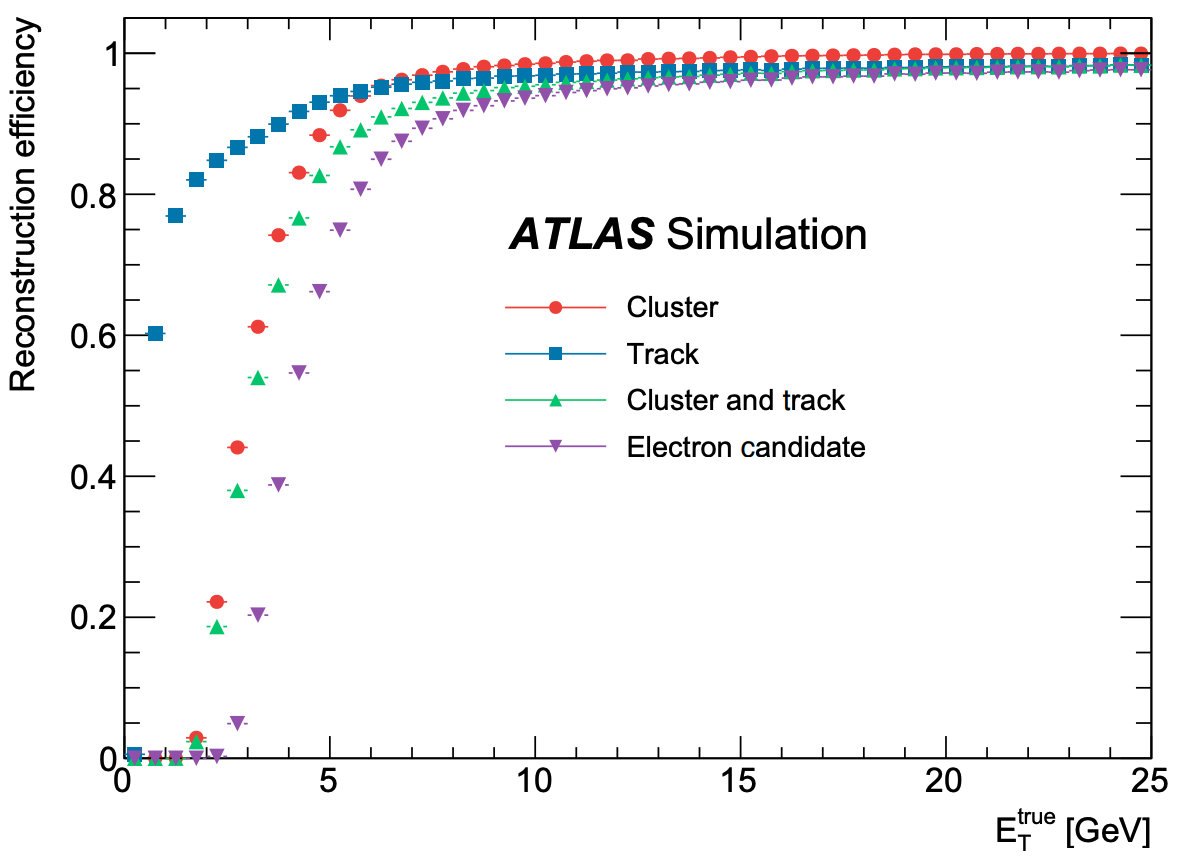
\includegraphics[width=.65\textwidth]{chapters/chapter3_eventreco/images/electron-efficiency.png}

    \caption[The reconstruction efficiency for electrons as a function of true \et.]{The reconstruction efficiency for electrons as a function of true \et for a single-electron sample. Each step of the candidate formation is shown \cite{electron-efficiency}.}
    \label{fig:electron-eff}
\end{figure}

\noindent\textbf{Track Reconstruction}\\ %https://arxiv.org/pdf/1902.04655.pdf
\indent Tracks are constructed out of hits within the \gls{ID}, in which three dimensional space-points are constructed out of clustered hits. Three sets of space-points are formed into track seeds, which then undergo stages of pattern recognition, ambiguity resolution, and \gls{TRT} extension. Track candidates with $\pt > \unit{400}{\MeV}$ are fit with the ATLAS Global $\chi^2$ fitter \cite{chi-2-fitter}. This uses the pion hypothesis for energy loss, however to accommodate for the bremsstrahlung losses, a second fit is performed using the electron hypothesis.

For tracks with at least four silicon hits that match to an \gls{EM} cluster, a secondary fit is performed using a Gaussian-sum filter \cite{gaussian-sum-filter}. This filter is is a generalization of the Kalman filter \cite{kalman-filter}, taking into account non-linearities resulting from bremsstrahlung radiation. The track perigee is then used to extrapolate to the \gls{EM} cluster in the second layer of the calorimeter, and must satisfy the following matching criteria to the cluster barycenter:
\begin{itemize}
    \item $|\eta_{cluster} - \eta_{track}| < 0.05$
    \item One of two azimuthal requirements:
    \begin{description}
        \item $-0.20 < \Delta \phi < 0.05$ for $\Delta \phi = -q \times (\phi_{cluster}-\phi_{track})$
        \item $-0.10 < \Delta \phi_{res} < 0.05$ for $\Delta \phi_{res}$ with the same definition as $\Delta \phi$,but the track momentum rescaled to the energy of the cluster
    \end{description}
\end{itemize}

%Figure \ref{fig:electron-eff} also shows the track reconstruction efficiency (blue), which is greater than 80\% efficient as low as $\et = \unit{1}{GeV}$, and more than 98\% efficient above $\et = \unit{10}{\GeV}$.




\subsection{Jets} \label{ssec:jet-reco}
As discussed in Section \ref{ssec:fermions}, strongly interacting particles cannot exist independently due to color confinement. Due to this, partons created in $pp$ collisions shower, a process where quarks radiating gluons and gluons split, ultimately creating a proliferation of subsequent partons. Ultimately, once they've reached a sufficiently low energy, about $\unit{1}{\GeV}$, they hadronize in order to create a colorless state, such as mesons or baryons that deposits energy into the calorimeters. This spray of interactions, both the showering and hadronization, all proceed in the general same direction and location, known as a ``jet.''

In principle, jets can be built from any set of 4-vector objects. For this work, they are constructed via topological clusters, described in detail in \ref{ssec:em-signatures}. Two classes of jet definitions exist. The first is cluster-based, which defines the jet by combining sets of four-vector objects until the distance between objects surpasses a stopping condition. The second is cone-based, which define jets as the sum of momenta within a defined radius, realizing jets as energy flow in a specified direction. ATLAS uses one such cone-based algorithm, known as the Anti-$k_t$ algorithm \cite{anti-kt}. The cone is built from topological clusters using a fixed radius, $R=0.4$\footnote{In analyses that probe high mass regimes, two jets may be overlapping and merge to produce one single large radius jet. This is known as a ``boosted'' topology, where the radius parameter is typically $R=1.0$. The presented analysis is not sensitive at high mass, thus such topologies are not considered.}. Since there is no a priori assumption on how fragmentation proceeds, jets are entirely defined via their algorithm.


Since all fragmenting strongly interacting particles appear as jets in the detector, an important process is \textit{flavor tagging}, which aims to classify the type of particle that produced a given jet. Paramount to the presented analysis is the process of $b$-tagging\footnote{In addition to $b$-tagging, ATLAS has also produced discriminators for charm jets ($c$-tagging).}, algorithms to classify jets which come from $b$-quarks. There are several algorithms to perform this classification, notably a \gls{BDT} named MV2 \cite{mv2-dl1} and a feed-forward deep \gls{NN}\footnote{See Appendix \ref{app:MVA} for an explanation of these multivariate techniques.} \cite{mv2-dl1}. From this score, $b$-tagging working points are established and calibrated based on their identification efficiency. 


\subsection{Muons} \label{ssec:muon-reco}
%http://cds.cern.ch/record/2139897/files/arXiv:1603.05598.pdf

Muons are a minimum-ionizing particle, leaving very little energy in the calorimeter, and are not stopped by any of the material in ATLAS. Thus, muons are reconstructed using a combination of track-based information from the \gls{ID} and the \gls{MS}. In the \gls{ID} tracks for muons is identical to other charged particles, outlined in Section \ref{ssec:em-signatures}. In the \gls{MS}, in each detector region (i.e. \glspl{MDT}, \glspl{CSC}, etc.), track segments are built from aligned hits in the bending plane of the detector, found via a Hough transform \cite{hough-transf}. Track candidates are formed by fitting together hits from different track segments via a combinatorial search outlined in Reference \cite{muon-reco}. Then an overlap removal algorithm finds the optimum track assignment. Ultimately hits are fitted with a global $\chi^2$ fit. Afterwards a hit recovery and subsequent track refit are performed if necessary.

Ultimately four muon types are defined \cite{muon-reco}:
\begin{itemize}
    \item Combined (CB) muon: Tracks reconstructed in the \gls{ID} are formed into a combined track using a global refit incorporating hits from both subdetectors.
    \item Segment-tagged (ST) muon: An \gls{ID} track is extrapolated to a local track segment in the \gls{MDT} or \gls{CSC}, accounting for muons that only cross one layer of \gls{MS} chambers.
    \item Calorimeter-tagged (CT) muon: An \gls{ID} track matched to a energy deposit in the calorimeter compatible with a minimum-ionizing particle. This muon type compensates for portions of the \gls{MS} that are only partially instrumented, near $\abseta \approx 0$.
    \item Extrapolated (ME) muons: These use only track information from the \gls{MS}, where parameters must be loosely in agreement with the location of the \gls{IP}. ME muons are useful for acceptance in $2.5 < \abseta < 2.7$, which is uncovered by the \gls{ID}.
\end{itemize}


From these muons, four selections are created (\textit{Loose}, \textit{Medium}, \textit{Tight}, and \textit{High-\pt}). These are defined based on varying requirements on the type of muon considered, number of hits, $\chi^2$ fit, $\eta$, $q/p$ \textit{significance}, and \pt. The efficiencies for the \textit{Loose} and \textit{Medium} selections are $>98\%$, and the \textit{Tight} selection ranges from $90\%$ to $98\%$ efficient. Figure \ref{fig:muon-eff} shows these efficiencies as a function of $\eta$.


\begin{figure}[!thp]
    \centering
    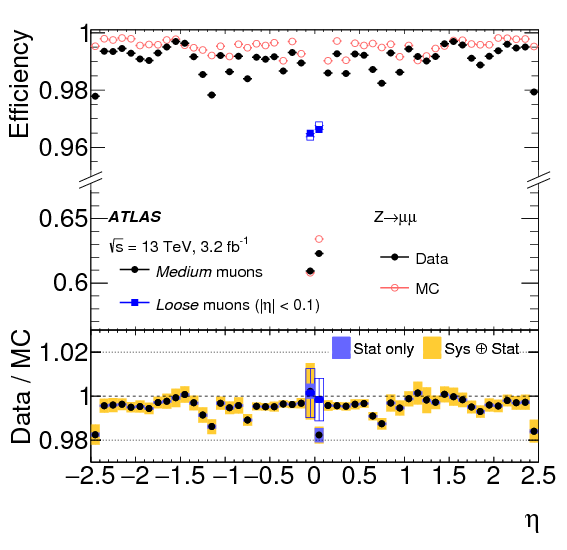
\includegraphics[width=.48\textwidth]{chapters/chapter3_eventreco/images/muon-medium.png}
    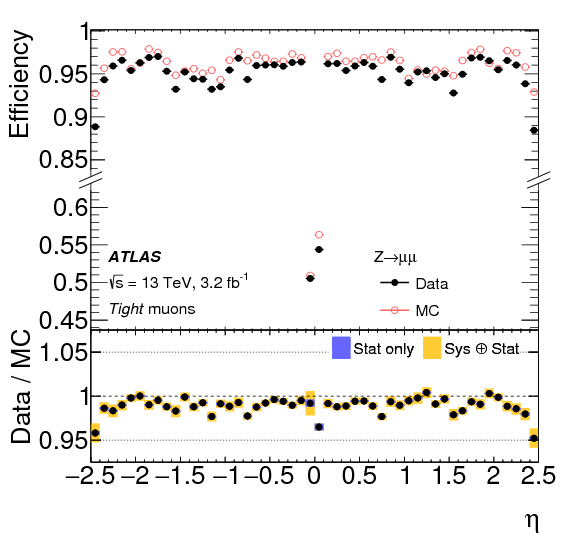
\includegraphics[width=.48\textwidth]{chapters/chapter3_eventreco/images/muon-tight.png}

    \caption[The reconstruction efficiency for \textit{Loose} and \textit{Tight} muons with $\pt >\unit{10}{\GeV}$ as a function of $\eta$.]
    {The reconstruction efficiency for muons with $\pt >\unit{10}{\GeV}$ as a function of $\eta$. The left panel shows the \textit{Loose} selection, the right shows the \textit{Tight} selection \cite{muon-reco}.}
    \label{fig:muon-eff}
\end{figure}
